%
% spektraltheorie.tex
%
% (c) 2020 Prof Dr Andreas Müller, Hochschule Rapperswil
% 
\section{Spektraltheorie
\label{buch:section:spektraltheorie}}
\rhead{Spektraltheorie}
Aufgabe der Spektraltheorie ist, Bedingungen an eine Matrix $A$ und eine
\index{Spektraltheorie}
Funktion $f(z)$ zu finden, unter denen es möglich ist, $f(A)$ auf 
konsistente Art und Weise zu definieren.
Weiter müssen Methoden entwickelt werden, mit denen $f(A)$ berechnet
werden kann.
Für ein Polynom $p(z)$ ist $p(A)$ durch Einsetzen definiert.
Für Funktionen, die sich nicht durch ein Polynom darstellen lassen,
muss eine Approximation der Funktion durch Polynome verwendet werden.
Sei also $p_n(z)$ eine Folge von Polynomen, die als Approximation der
Funktion $f(z)$ verwendet werden soll.
Das Ziel ist, $f(A)$ als den Grenzwert der Matrixfolge $p_n(A)$
zu definieren.

Zunächst ist nicht klar, wie eine solche Folge gewählt werden muss.
Es muss eine Teilmenge von $K\subset\mathbb{C}$ spezifiziert werden,
auf der die Funktionenfolge $p_n(z)$ konvergieren muss,
damit auch die Konvergenz der Matrizenfolge $p_n(A)$ garantiert ist.
Auch die Art der Konvergenz von $p_n(z)$ auf der Menge $K$ ist noch
unklar.
Da der Abstand zweier Matrizen $A$ und $B$ in der Operatornorm
mit der grössten Abweichung $\|(A-B)v\|$ für Einheitsvektoren $v$
gemessen wird, ist es einigermassen plausibel, dass
die grösste Abweichung zwischen zwei Polynomen $|p(z) - q(z)|$ auf
der Menge $K$ klein sein muss, wenn $\|p(A)-q(A)\|$ klein 
sein soll.
Da die Differenz $p(z)-q(z)$ für beliebige Polynome, die sich nicht
nur um eine Konstante unterscheiden, mit $z$ über alle Grenzen wächst,
muss $K$ beschränkt sein.
Gesucht ist also eine kompakte Menge $K\subset\mathbb{C}$ und eine
Folge $p_n(z)$ von Polynomen, die auf $K$ gleichmässig gegen $f(z)$
konvergieren.
Die Wahl von $K$ muss sicherstellen, dass für jede gleichmässig
konvergente Folge von Polynomen $p_n(z)$ auch die Matrizenfolge
$p_n(A)$ konvergiert.

Es wird sich zeigen, dass die Menge $K$ das Spektrum von $A$ ist,
$K=\operatorname{Sp}(A)$,
(Definition~\ref{buch:eigenwerte:def:spektrum}),
also eine endliche Teilmenge von $\mathbb{C}$.
\index{Spektrum}
Jede Funktion kann auf so einer Menge durch Polynome exakt wiedergegeben
werden.
Es gibt insbesondere Folgen von Polynomen, die eingeschränkt
auf das Spektrum gleich sind, also $p_n(z)=p_m(z)$ für alle $z\in K$,
die aber ausserhalb des Spektrums alle verschieden sind.
Als Beispiel kann die Matrix 
\[
N=\begin{pmatrix}0&1\\0&0\end{pmatrix}
\]
herangezogen werden.
Ihr Spektrum ist $\operatorname{Sp}(N)=\{0\}\subset\mathbb{C}$.
Zwei Polynome stimmen genau dann auf $\operatorname{Sp}(N)$ überein,
wenn der konstante Koeffizient gleich ist.
Die Polynome $p(z)=z$ und $q(z)=z^2$ stimmen daher auf dem Spektrum
überein.
Für die Matrizen gilt aber $p(N)=N$ und $q(N)=N^2=0$, die Matrizen
stimmen also nicht überein.
Es braucht also zusätzliche Bedingungen an die Matrix $A$, die
sicherstellen, dass $p(A)=0$ ist, wann immer $p(z)=0$ für
$z\in\operatorname{Sp}(A)$ gilt.

In diesem Abschnitt sollen diese Fragen untersucht werden.
In Abschnitt~\ref{buch:subsection:approximation-durch-polynome}
wird gezeigt, wie sich Funktionen durch Polynome approximieren
lassen, woraus sich dann Approximationen von $f(A)$ für diagonalisierbare
Matrizen mit reellen Eigenwerten ergeben.

Der Satz von Stone-Weierstrass, der in
\index{Stone-Weierstrass, Satz von}%
\index{Satz von Stone-Weierstrass}%
Abschnitt~\ref{buch:subsetion:stone-weierstrass} dargestellt wird,
ist ein sehr allgemeines Approximationsresultat, welches nicht nur
zeigt, dass die Approximation unter einigermassen natürlichen Voraussetzungen
beliebig genau möglich ist, sondern uns im komplexen Fall auch
weitere Einsicht in die Voraussetzungen an eine
komplexe Matrix geben kann, damit man damit rechnen kann,
dass die Approximation zu einer konsistenten Definition von $f(A)$ führt.

%
% Approximation
%
\subsection{Approximation durch Polynome
\label{buch:subsection:approximation-durch-polynome}}
Die der Berechnung von $f(A)$ für eine beleibige stetige Funktion,
die sich nicht als Potenzreihe schreiben lässt, verwendet Approximationen
von Polynomen.
Die numerische Mathematik hat eine grosse Menge von solchen
Approximationsverfahren entwickelt, wovon zwei kurz (ohne Beweise)
vorgestellt werden sollen.

\subsubsection{Das Legendre-Interpolationspolynom}
\index{Legendre-Interpolationspolynom}%
Zu vorgegebenen, verschiedenen Zahlen $z_i\in\mathbb{C}$, $0\le i\le n$,
die auch die {\em Stützstellen} genannt werden,
\index{Stützstelle}%
gibt es immer ein Polynom vom Grade $n$, welches in den $z_i$ vorgegebene
Werte $f(z_i)$ annimmt.
Ein solches Polynom lässt sich im Prinzip mit Hilfe eines linearen
Gleichungssystems finden, man kann aber auch direkt eine Lösung
konstruieren.
Dazu bildet man erst die Polynome
\begin{align*}
l(z) &= (z-z_0)(z-z_1)\cdots (z-z_n) \qquad\text{und}
\\
l_i(z) &= (z-z_0)\cdots \widehat{(z-z_i)}\cdots (z-z_n).
\end{align*}
Darin bedeutet der Hut, dass dieser Term weggelassen werden soll.
Für $z\ne z_i$ ist $l_i(z)=l(z)/(z-z_i)$.
Die Polynome
\[
k_i(z)
=
\frac{l_i(z)}{l_i(z_i)}
=
\frac{(z-z_0)\cdots \widehat{(z-z_i)}\cdots (z-z_n)}{(z_i-z_0)\cdots \widehat{(z_i-z_i)}\cdots (z_i-z_n)}
\]
haben die Eigenschaft
$k_i(z_j)=\delta_{i\!j}$.
Damit lässt sich jetzt ein Polynom
\[
p(z) = \sum_{j=0}^n f(z_j) \frac{l_j(z)}{l_j(z_j)}
\]
vom Grad $n$ konstruieren, welches die Werte
\[
p(z_i)
=
\sum_{j=0}^n f(z_j) \frac{l_j(z_i)}{l_j(z_j)}
=
\sum_{j=0}^n f(z_j) \delta_{i\!j}
=
f(z_i)
\]
annimmt.
Das Polynom $p(z)$ heisst das {\em Legendre-Interpolationspolynom}.

Zwar lässt sich auf diese Weise für eine endliche Menge von komplexen Zahlen
immer ein Polynom finden, welches vorgeschriebene Wert in allen diesen Zahlen
annimmt, doch ist die Stabilität für grosse $n$ eher schlecht.


\subsubsection{Gleichmassige Approximation mit Bernstein-Polynomen}
\index{Bernstein-Polynom}%
Das Legendre-Interpolationspolynom nimmt in den  Stützstellen die
verlangten Werte an, aber ausserhalb der Stützstellen ist nicht
garantiert, dass man eine gute Approximation einer Funktion $f(z)$
erhält.
Für die Approximation auf einem reellen Interval $[a,b]$ hat
Sergei Natanowitsch Bernstein eine Methode zur expliziten
Konstruktion eines Approximationspolynoms formuliert.

Dazu werden zuerst die reellen Bernsteinpolynome vom Grad $n$
durch
\begin{align*}
B_{i,n}(t) = \binom{n}{i} t^i(1-t)^{n-i}
\end{align*}
definiert.
Als Approximationspolynom für die auf dem Interval 
$[0,1]$ definierte, stetige Funktion $f(t)$ kann man dann
\[
B_n(f)(t)
=
\sum_{i=0}^n B_{i,n}(t) f\biggl(\frac{i}{n}\biggr)
\]
verwenden.
Die Polynome $B_n(f)(t)$ konvergieren gleichmässig auf $[0,1]$
gegen die Funktion $f(t)$.
Über die Konvergenz ausserhalb des reellen Intervalls wird nichts
ausgesagt.
Die Approximation mit Bernstein-Polynomen ist daher nur sinnvoll,
wenn man weiss, dass die Eigenwerte der Matrix reell sind.

Für ein anderes Interval $[a,b]$ kann man ein Approximationspolynom
erhalten, indem man die affine Transformation
$s\mapsto (s-a)/(b-a)$
von $[a,b]$ auf $[0,1]$
verwendet. 

%
% Der Satz von Stone-Weierstrass
%
\subsection{Der Satz von Stone-Weierstrasss
\label{buch:subsetion:stone-weierstrass}}
\index{Stone-Weierstrass, Satz von}%
\index{Satz von Stone-Weierstrass}%
Der Satz von Stone-Weierstrass behandelt im Gegensatz zu den in
Abschnitt~\ref{buch:subsection:approximation-durch-polynome}
besprochenen Approximationsmethoden nicht nur Funktionen von
reellen Variablen durch Polynome.
Vielmehr kann das Definitionsgebiet irgend eine abgeschlossene
und beschränkte Teilmenge eines reellen oder komplexen Vektorraumes
sein und die Funktionen können Polynome aber auch viel allgemeinere
Funktionen verwendet werden, wie zum Beispiel die Funktionen
$x\mapsto \cos nx$ und $x\mapsto \sin nx$ definiert auf dem
Intervall $[0,2\pi]$.
In diesem Fall liefert der Satz von Stone-Weierstrass die Aussage,
dass sich jede stetige periodische Funktion gleichmässig durch
trigonometrische Polynome approximieren lässt.

Die Aussage des Satzes von Stone-Weierstrass über reelle Funktionen
lässt sich nicht auf komplexe Funktionen erweitern.
Von besonderem Interesse ist jedoch, dass der Beweis des Satz 
zeigt, warum solche Aussagen für komplexe Funktionen nicht mehr
zutreffen.
Im Falle der Approximation von komplexen Funktionen $f(z)$ durch Polynome
zwecks Definition von $f(A)$ werden sich daraus Bedingungen an die
Matrix ableiten lassen, die eine konsistente Definition überhaupt
erst ermöglichen werden.

\subsubsection{Punkte trennen}
Aus den konstanten Funktionen lassen sich durch algebraische
Operationen nur weitere konstante Funktionen erzeugen.
Die konstanten Funktionen sind also nur dann eine genügend
reichhaltige Menge für die Approximation von Funktionen auf $K$,
wenn die Menge $K$ nur einen einzigen Punkt enthält.
Damit sich Funktionen approximieren lassen, die in zwei Punkten
verschiedene Werte haben, muss es auch unter den zur Approximation
zur Verfügung stehenden Funktionen solche haben, deren Werte sich
in diesen Punkten unterscheiden.
Diese Bedingung wird in der folgenden Definition formalisiert.

\begin{definition}
Sei $K$ eine beliebige Menge und $A$ eine Menge von Funktionen
$K\to \mathbb{C}$.
Man sagt, $A$ {\em trennt die Punkte von $K$}, wenn es für jedes Paar
\index{Punkte trennen}%
von Punkten $x,y\in K$ eine Funktion $f\in A$ gibt derart, dass
$f(x)\ne f(y)$.
\end{definition}

Man kann sich die Funktionen $f$, die gemäss dieser Definition die Punkte
von $K$ trennen, als eine Art Koordinaten der Punkte in $K$ vorstellen.
Die Punkte der Teilmenge $K\subset \mathbb{R}^n$ werden zum Beispiel
von den Koordinatenfunktionen $x\mapsto x_i$ getrennt.
Wir schreiben für die $i$-Koordinate daher auch als Funktion $x_i(x)=x_i$.
Zwei verschiedene Punkte $x,y\in K$ unterscheiden sich in mindestens
einer Koordinate.
Für diese Koordinate sind dann die Werte der zugehörigen
Koordinatenfunktion $x_i=x_i(x)\ne x_i(y)=y_i$ verschieden, die
Funktionen $x_1(x)$ bis $x_n(x)$ trennen also die Punkte.

\begin{beispiel}
Wir betrachten einen Kreis in der Ebene, also die Menge
\[
S^1
=
\{(x_1,x_2) \mid x_1^2 + x_2^2=1\}
\]
$S^1$ ist eine abgeschlossene und beschränkte Menge in $\mathbb{R}^2$.
Die Funktion $x\mapsto x_1$ trennt die Punkte nicht, denn zu jedem
Punkt $(x_1,x_2)\in S^2$ gibt es den an der ersten Achse
gespiegelten Punkt $\sigma(x)=(x_1,-x_2)$, dessen erste Koordinate
den gleichen Wert hat.
Ebenso trennt die Koordinatenfunktion $x\mapsto x_2$ die Punkte nicht.
Die Menge $A=\{ x_1(x), x_2(x)\}$ bestehend aus den beiden
Koordinatenfunktionen trennt dagegen die Punkte von $S^1$, da die Punkte
sich immer in mindestens einem Punkt unterscheiden.

Man könnte auch versuchen, den Kreis in Polarkoordinaten zu beschreiben.
Die Funktion $\varphi(x)$, die jedem Punkt $x\in S^1$ den Polarwinkel
zuordnet, trennt sicher die Punkte des Kreises.
Zwei verschiedene Punkte auf dem Kreis haben verschieden Polarwinkel.
Die Menge $\{\varphi\}$ trennt also die Punkte von $S^1$.
Allerdings ist die Funktion nicht stetig, was zwar der Definition
nicht widerspricht aber ein Hindernis für spätere Anwendungen ist.
\end{beispiel}


\subsubsection{Der Satz von Stone-Weierstrass für reelle Funktionen}
\index{Satz von Stone-Weierstrass}%
\index{Stone-Weierstrass, Satz von}%
Die Beispiele von Abschnitt~\ref{buch:subsection:approximation-durch-polynome}
haben bezeigt, dass sich reellwertige Funktionen einer reellen
Variable durch Polynome beliebig genau approximieren lassen.
Es wurde sogar eine Methode vorgestellt, die eine auf einem Intervall
gleichmässig konvergente Polynomefolge produziert.
Die Variable $x\in[a,b]$ trennt natürlich die Punkte, die Algebra der
Polynome in der Variablen $x$ enthält also sicher Funktionen, die in
verschiedenen Punkten des Intervalls auch verschiedene Werte annehmen.
Nicht ganz so selbstverständlich ist aber, dass sich daraus bereits
ergibt, dass jede beliebige Funktion sich durch Polynome in $x$
approximieren lässt.
Dies ist der Inhalt des folgenden Satzes von Stone-Weierstrass.

\begin{figure}
\centering
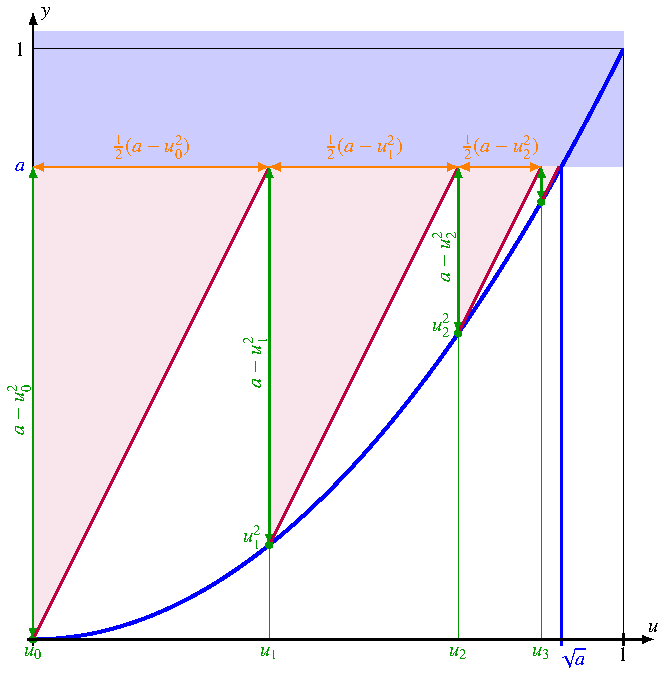
\includegraphics{chapters/40-eigenwerte/images/wurzel.pdf}
\caption{Konstruktion einer monoton wachsenden Approximationsfolge für
$\sqrt{a}$
\label{buch:eigenwerte:fig:wurzelverfahren}}
\end{figure}

\begin{figure}
\centering
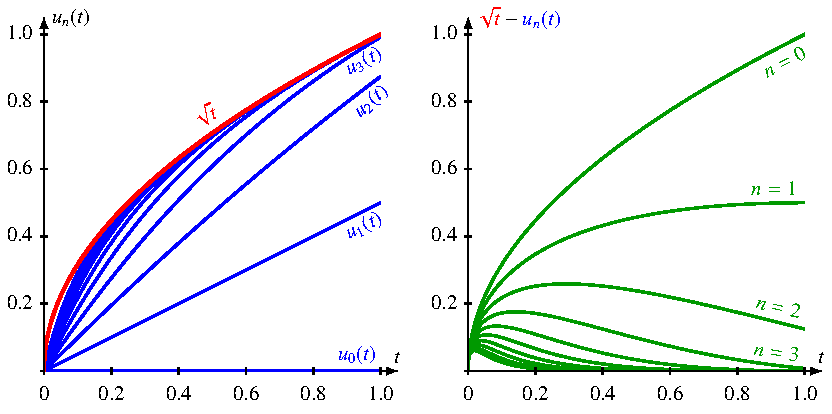
\includegraphics[width=\textwidth]{chapters/40-eigenwerte/images/wurzelapprox.pdf}
\caption{Monoton wachsende Approximation der Funktion $t\mapsto\sqrt{t}$ mit 
Polynomen $u_n(t)$ nach 
\eqref{buch:eigenwerte:eqn:wurzelapproximation}
(links) und der Fehler der Approximation
(rechts).
\label{buch:eigenwerte:fig:wurzelapproximation}}
\end{figure}

\begin{satz}[Stone-Weierstrass]
\label{buch:satz:stone-weierstrass}
Enthält eine $\mathbb{R}$-Algebra $A$ von stetigen, rellen Funktionen
auf einer kompakten Menge $K$ die konstanten Funktionen und trennt sie
Punkte, d.~h.~für zwei verschiedene Punkte $x,y\in K$ gibt es
immer eine Funktion $f\in A$ mit $f(x)\ne f(y)$, dann ist jede stetige,
reelle Funktion auf $K$ gleichmässig approximierbar durch Funktionen 
in $A$.
\end{satz}

Für den Beweis des Satzes wird ein Hilfsresultat benötigt, welches wir
zunächst ableiten.
Es besagt, dass sich die Wurzelfunktion $t\mapsto\sqrt{t}$
\index{Wurzelfunktion}%
auf dem Interval $[0,1]$ gleichmässig
von unten durch Polynome approximieren lässt, die in
Abbildung~\ref{buch:eigenwerte:fig:wurzelapproximation} dargestellt
sind.

\begin{satz}
Die rekursiv definierte Folge von Polynomen
\begin{equation}
u_{n+1}(t)
=
u_n(t) + \frac12(t-u_n(t)^2),
\qquad
u_0(t)=0
\label{buch:eigenwerte:eqn:wurzelapproximation}
\end{equation}
ist monoton wachsend und approximiert die Wurzelfunktion $t\mapsto\sqrt{t}$
gleichmässig auf dem Intervall $[0,1]$.
\end{satz}

\begin{figure}
\centering
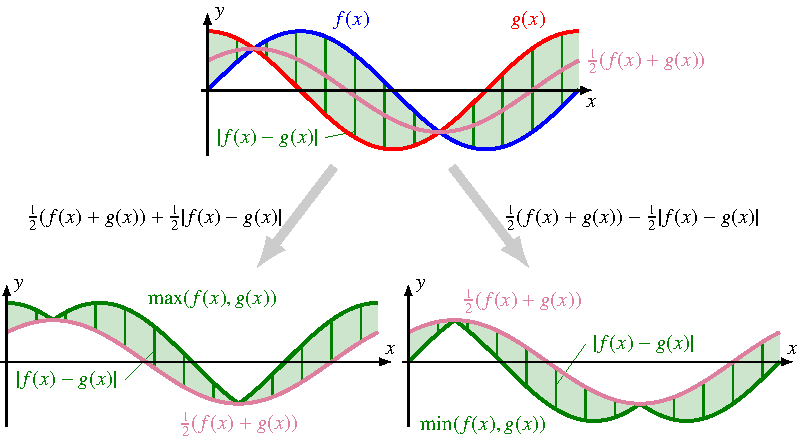
\includegraphics{chapters/40-eigenwerte/images/minmax.pdf}
\caption{Graphische Erklärung der
Identitäten~\eqref{buch:eigenwerte:eqn:minmax} für
$\max(f(x),g(x))$ und $\min(f(x),g(x))$.
Die purpurrote Kurve stellt den Mittelwert von $f(x)$ und $g(x)$ dar,
die vertikalen grünen Linien haben die Länge der Differenz $|f(x)-g(x)|$.
Das Maximum erhält man, indem man den halben Betrag der Differenz zum
Mittelwert hinzuaddiert, das Minimum erhält man durch Subtraktion
der selben Grösse.
\label{buch:eigenwerte:fig:minmax}}
\end{figure}

\begin{proof}[Beweis]
Wir konstruieren zunächst das in
Abbildung~\ref{buch:eigenwerte:fig:wurzelverfahren}
visualisierte Verfahren, mit dem für jede Zahl $a\in[0,1]$
die Wurzel $\sqrt{a}$ berechnet werden kann.
Sei $u < \sqrt{a}$ eine Approximation der Wurzel.
Die Approximation ist der exakte Wert, wenn $a-u^2=0$.
In jedem anderen Fall muss $u$ um einen Betrag $d$ vergrössert werden.
Natürlich muss immer noch $u+d<\sqrt{a}$ sein.
Man kann die maximal zulässige Korrektur $d$ geometrisch abschätzen,
wie dies in Abbildung~\ref{buch:eigenwerte:fig:wurzelverfahren}
skizziert ist.
Die maximale Steigung des Graphen der Funktion $u\mapsto u^2$ ist $2$,
daher darf man $u$ maximal um die Hälfte der Differenz $a-u^2$ (grün)
vergrössern, also $d=\frac12(a-u^2)$.
Die Rekursionsformel
\[
u_{n+1} = u_n + d = u_n + \frac12(a-u_n^2)
\]
mit dem Startwert $u_0=0$ liefert daher eine 
Folge, die gegen $\sqrt{a}$ konvergiert.
\end{proof}

\begin{proof}[Beweis des Satzes von Stone-Weierstrass]
\index{Stone-Weierstrass, Beweis}%
\index{Satz von Stone-Weierstrasse, Beweis}%
Da $A$ eine Algebra ist, ist mit jeder Funktion $f\in A$ für jedes Polynome
$p\in\mathbb{R}[X]$ auch $p(f)$ eine Funktion in $A$.
\begin{enumerate}
\item Schritt: Für jede Funktion $f\in A$ lässt sich auch $|f|$ durch
Funktionen in $A$ beliebig genau durch eine monoton wachsende Folge
von Funktionen approximieren.

Da $A$ eine Algebra ist, ist $f^2\in A$.
Sei ausserdem $m^2=\sup \{f(x)^2 \mid x\in K\}$, so dass $f^2/m^2$ eine Funktion
mit Werten im Intervall $[0,1]$ ist.
Die Funktionen $f_n(x)=mu_n(f(x)^2/m^2)$ sind ebenfalls in $A$,
bilden eine monoton wachsende Folge von Funktionen und
approximieren $\sqrt{f(x)^2}=|f(x)|$ gleichmässig.

\item Schritt: Für zwei Funktionen $f,g\in A$ gibt es eine monoton wachsende
Folge, die $\max(f,g)$ gleichmässig beliebig genau approximiert
und eine monoton fallende Folge, die $\min(f,g)$ gleichmässig beliebig 
genau approximiert.

Diese Folgen können aus der Approximationsfolge für den Betrag einer
Funktion und den Identitäten
\begin{equation}
\begin{aligned}
\max(f,g) &= \frac12(f+g+|f-g|) \\
\min(f,g) &= \frac12(f+g-|f-g|) 
\end{aligned}
\label{buch:eigenwerte:eqn:minmax}
\end{equation}
gefunden werden, die in Abbildung~\ref{buch:eigenwerte:fig:minmax}
graphisch erklärt werden.

\item Schritt: Zu zwei beliebigen Punkten $x,y\in K$ und Werten
$\alpha,\beta\in\mathbb{R}$ gibt es immer eine Funktion in $A$,
die in den Punkten $x,y$ die vorgegebenen Werte $\alpha$ bzw.~$\beta$
annimmt.
Da $A$ die Punkte trennt, gibt es eine Funktion $f_0$ mit $f_0(x)\ne f_0(y)$.
Dann ist die Funktion
\[
f(t)
=
\beta + \frac{f_0(t)-f_0(y)}{f_0(x)-f_0(y)}(\alpha-\beta)
\]
wohldefiniert, liegt in $A$ und nimmt die verlangten Werte an.

\item Schritt: Zu jeder stetigen Funktion $f\colon K\to\mathbb{R}$, jedem
Punkt $x\in K$ und jedem $\varepsilon>0$ gibt es eine Funktion $g\in A$ derart,
dass $g(x)=f(x)$ und $g(y) \le f(y)+\varepsilon$ für alle $y\in K$.

Zu jedem $z\in K$ gibt es eine Funktion $h_z\in A$ mit
$h_z(x)=f(x)$ und $h_z(z) \le f(z)+\frac12\varepsilon$.
Wegen der Stetigkeit von $h_z$ gibt es eine Umgebung $V_z$ von $z$, in der
immer noch gilt $h_z(y)\le f(y)+\varepsilon$ für $y\in V_z$.
Wegen der Kompaktheit von $K$ kann man endlich viele Punkte $z_i$ wählen
derart, dass die $V_{z_i}$ immer noch $K$ überdecken.
Dann erfüllt die Funktion
\(
g(z) = \inf h_{z_i}
\)
die Bedingungen $g(x) = f(x)$ und für $z\in V_{z_i}$
\[
g(z) = \inf_{j} h_{z_j}(z) \le h_{z_i}(z) \le f(z)+\varepsilon.
\]
Ausserdem ist $g(z)$ nach dem zweiten Schritt beliebig genau durch
Funktionen in $A$ approximierbar.
\item Schritt: Jede stetige Funktion $f\colon K\to\mathbb{R}$ kann
beliebig genau durch Funktionen in $A$ approximiert werden.

Sei $\varepsilon > 0$.
Nach dem vierten Schritt gibt es für jedes $y\in K$ eine Funktion $g_y$
derart, dass $g_y(y)=f(y)$  und $g_y(x) \le f(x) + \varepsilon$ für
$x\in K$.
Da $g_y$ stetig ist, gilt ausserdem $g_y(x) \ge f(x) -\varepsilon$ in
einer Umgebung $U_y$ von $y$.
Da $K$ kompakt ist, kann man endlich viele $y_i$ derart wählen,
dass die $U_{y_i}$ immer noch ganz $K$ überdecken.
Die Funktion $g=\sup g_{y_i}$ erfüllt dann überall $g(x) \le f(x)+\varepsilon$,
weil jede der Funktionen $g_y$ diese Ungleichung erfüllt.
Ausserdem gilt für $x\in V_{x_j}$
\[
g(x) = \sup_i g_{x_i}(x) \ge g_{x_j}(x) \ge f(x)-\varepsilon.
\]
Somit ist
\[
|f(x)-g(x)| \le \varepsilon.
\]
Damit ist $f(x)$ beliebig nahe an der Funktion $g(x)$, die sich 
beliebig genau durch Funktionen aus $A$ approximieren lässt.
\qedhere
\end{enumerate}
\end{proof}

Im ersten Schritt des Beweises ist ganz entscheidend, dass man die
Betragsfunktion konstruieren kann.
Daraus leiten sich dann alle folgenden Konstruktionen ab.

\subsubsection{Anwendung auf symmetrische und hermitesche Matrizen}
Für symmetrische und hermitesche Matrizen $A$ ist bekannt, dass die
Eigenwerte reell sind, also das Spektrum $\operatorname{A}\subset\mathbb{R}$
ist.
Für eine Funktion $\mathbb{R}\to \mathbb{R}$ lässt sich nach dem
Satz~\ref{buch:satz:stone-weierstrass} immer eine Folge $p_n$ von
approximierenden Polynomen in $x$ finden, die auf $\operatorname{Sp}(A)$
gleichmässig konvergiert.
Die Matrix $f(A)$ kann dann definiert werden also der Grenzwert
\[
f(A) = \lim_{n\to\infty} p_n(A).
\]
Da diese Matrizen auch diagonalisierbar sind, kann man eine Basis
aus Eigenvektoren verwenden.
Die Wirkung von $p_n(A)$ auf einem Eigenvektor $v$ zum Eigenwert $\lambda$
ist
\[
p_n(A)v
=
(a_kA^k + a_{k-1}A^{k-1}+\dots +a_2A^2+a_1A+a_0I)v
=
(a_k\lambda^k + a_{k-1}\lambda^{k-1}+\dots + a_2\lambda^2 + a_1\lambda + a_0)v
=
p_n(\lambda)v.
\]
Im Grenzwert wirkt $f(A)$ daher durch Multiplikation eines Eigenvektors
mit $f(\lambda)$, die Matrix $f(A)$ hat in der genannten Basis die
Diagonalform
\[
A=\begin{pmatrix}
\lambda_1&         &      &         \\
         &\lambda_2&      &         \\
         &         &\ddots&         \\
         &         &      &\lambda_n
\end{pmatrix}
\qquad\Rightarrow\qquad
f(A)=\begin{pmatrix}
f(\lambda_1)&            &      &            \\
            &f(\lambda_2)&      &            \\
            &            &\ddots&            \\
            &            &      &f(\lambda_n)
\end{pmatrix}.
\]

Insgesamt haben wir damit den folgenden {\em Spektralsatz } für symmetrische
und hermitesche Matrizen erhalten.
\index{Spektralsatz}%

\begin{satz}[Spektralsatz]
\label{buch:eigenwerte:satz:spektralsatz}
\index{symmetrische Matrix}%
\index{Matrix, symmetrisch}%
\index{hermitesche Matrix}%
\index{Matrix, hermitesche}%
Ist $A$ symmetrische oder hermitesche Matrix und $f$ eine Funktion
auf dem Spektrum $\operatorname{Sp}(A)$ von $A$.
Dann gibt es genau eine Matrix $f(A)$, die Grenzwert jeder beliebigen
Folge $p_n(A)$ mit Polynomen $p_n(x)$ ist, die auf $\operatorname{Sp}(A)$
gleichmässig gegen $f$ konvergieren.
\end{satz}

\subsubsection{Unmöglichkeit der Approximation von $z\mapsto \overline{z}$
in $\mathbb{C}[z]$}
Der Satz~\ref{buch:satz:stone-weierstrass} von Stone-Weierstrass für
reelle Funktionen gilt nicht für komplexe Funktionen.
In diesem Abschnitt zeigen wir, dass sich die Funktion $z\mapsto\overline{z}$
auf der Einheitskreisscheibe $K=\{z\in\mathbb{C} \mid |z|\le 1\}$ nicht
gleichmässig durch Polynome $p(z)$ mit komplexen Koeffizienten approximieren
lässt.
Sei also $p_n(z)$ eine Folge von Polynomen, die auf der Einheitskreisscheibe
gleichmässig gegen $\overline{z}$ konvergieren, also
$\overline{z}=\lim_{n\to\infty}p_n(z)$.

Das Wegintegral beider Seiten über den Pfad $\gamma(t) = e^{it}$
in der komplexen Ebene ist
\begin{align*}
\oint_\gamma z^k\,dz
&=
\int_0^{2\pi} e^{ikt} ie^{it}\,dt
=
i\int_0^{2\pi} e^{it(k+1)}\,dt
=
i\biggl[ \frac{1}{i(k+1)} e^{it(k+1)}\biggr]_0^{2\pi}
=
0
\\
\oint_\gamma
p(z)
\,dz
&=
\sum_{k=0}^\infty a_{n,k} \oint_\gamma z^k\,dz
=
\sum_{k=0}^\infty a_{n,k}\cdot 0
=
0
\\
\oint_\gamma \overline{z}\,dz
&=
\int_0^{2\pi} e^{it} ie^{it}\,dt
=
i\int_0^{2\pi} \,dt = 2\pi i,
\end{align*}
dabei wurde $\overline{\gamma}(t)=e^{-it}$ verwendet.
Insbesondere widersprechen sich die beiden Integrale.
Die ursprüngliche Annahme, $\overline{z}$ lasse sich durch Polynome
gleichmässig approximieren, muss daher verworfen werden.

\subsubsection{Der Satz von Stone-Weierstrass für komplexe Funktionen}
Der Satz von Stone-Weierstrass kann nach dem vorangegangene Abschnitt
für komplexe Funktionen nicht gelten, denn wir haben eine Funktion
gefunden, die sich nicht approximieren lässt.
Um den Beweis des Satzes~\ref{buch:satz:stone-weierstrass}
auf komplexe Zahlen zu übertragen, muss im ersten Schritt ein Weg
gefunden werden, den Betrag einer Funktion zu approximieren.

Im reellen Fall geschah dies, indem zunächst eine Polynom-Approximation
für die Quadratwurzel konstruiert wurde, die dann auf das Quadrat einer
Funktion angewendet wurde.
Der Betrag einer komplexen Zahl $z$ ist aber nicht allein aus $z$
berechenbar, man braucht in irgend einer Form Zugang zu Real-
und Imaginärteil.
Zum Beispiel kann man Real- und Imaginärteil als
$\Re z= \frac12(z+\overline{z})$ und $\Im z = \frac12(z-\overline{z})$
bestimmen.
Die Kenntnis von Real- und Imaginärteil ist gleichbedeutend mit
der Kenntnis der komplex Konjugierten $\overline{z}$.
Der Betrag lässt sich daraus als $|z|^2 = z\overline{z}$ finden.
Beide Beispiele zeigen, dass man den im Beweis benötigten Betrag
nur dann bestimmen kann, wenn mit jeder Funktion aus $A$ auch die
komplex konjugierte Funktion zur Verfügung steht.

\begin{satz}[Stone-Weierstrass]
\index{Satz von Stone-Weierstrass für komplexe Funktionen}
\index{Stone-Weierstrass, Satz für komplexe Funktionen}
Enthält eine $\mathbb{C}$-Algebra $A$ von stetigen, komplexwertigen
Funktionen auf einer kompakten Menge $K$ die konstanten Funktionen,
trennt sie Punkte und ist ausserdem mit jeder Funktion $f\in A$ auch
die komplex konjugiert Funktion $\overline{f}\in A$,
dann lässt sich jede stetige, komplexwertige Funktion 
auf $K$ gleichmässig durch Funktionen aus $A$ approximieren.
\end{satz}

Mit Hilfe der konjugiert komplexen Funktion lässt sich immer eine
Approximation für die Betragsfunktion finden, so dass sich der
Beweis des reellen Satzes von Stone-Weierstrass übertragen lässt.

%
% Normale Matrizen
%
\subsection{Normale Matrizen
\label{buch:subsection:normale-matrizen}}
Aus dem Satz von Stone-Weierstrass für komplexe Matrizen kann man
jetzt einen Spektralsatz für eine etwas grössere Klasse von Matrizen
\index{Spektralsatz}%
ableiten, als im Satz~\ref{buch:eigenwerte:satz:spektralsatz}
möglich war.
Der Satz besagt, dass für eine beliebige Funktion $f$ auf dem Spektrum
$\operatorname{Sp}(A)$ eine Folge von auf $\operatorname{Sp}(A)$
gleichmässig konvergenten, approximierenden Polynomen
$p_n(z,\overline{z})$ gefunden werden kann.
Doch wie soll jetzt aus dieser Polynomfolge ein Kandidat von $f(A)$
gefunden werden?

Zunächst stellt sich die Frage, was für die Variable $\overline{z}$ 
eingesetzt werden soll.
$1\times 1$-Matrizen sind notwendigerweise diagonal, also muss 
man in diesem Fall die Matrix $\overline{A}$ für die Variable
$\overline{z}$ eingesetzt werden.
Dies erklärt aber noch nicht, wie für $n\times n$-Matrizen
vorzugehen ist, wenn $n>1$ ist.

Die Notwendigkeit, die Variable $\overline{z}$ hinzuzunehmen,
ergab sich aus der Anforderung, dass der Betrag aus $|z|^2=z\overline{z}$
konstruiert werden können muss.
Insbesondere muss beim Einsetzen eine Matrix entstehen, die nur 
positive Eigenwerte hat.
Für eine beliebige komplexe $n\times n$-Matrix $A$ ist aber
$A\overline{A}$ nicht notwendigerweise positiv, wie das Beispiel
\[
A
=
\begin{pmatrix}0&i\\i&0\end{pmatrix}
\qquad
\Rightarrow
\qquad
A\overline{A}
=
\begin{pmatrix}0&i\\-i&0\end{pmatrix}
\begin{pmatrix}0&-i\\i&0\end{pmatrix}
=
\begin{pmatrix}
-1&0\\
 0&-1
\end{pmatrix}
=
-I
\]
zeigt.
Eine positive Matrix entsteht dagegen immer, wenn man statt
$A$ die hermitesche Konjugierte $A^*=\overline{A}^t$ verwendet.

Die Substitution von $A$ für $z$ und $A^*$ für $\overline{z}$
in einem Polynom $p(z,\overline{z})$ ist nicht unbedingt eindeutig.
Schon das Polynom $p(z,\overline{z})=z\overline{z}$ kann man auch
als $\overline{z}z$ schreiben.
Damit die Substitution eindeutig wird, muss man also fordern, dass
$AA^* = A^*A$ ist.

\begin{definition}
Eine Matrix $A\in M_n(\mathbb{C})$ heisst {\em normal}, wenn $AA^*=A^*A$ gilt.
\index{normal}%
\end{definition}

\subsubsection{Beispiele normaler Matrizen}

\begin{enumerate}
\item
Hermitesche und Antihermitesche Matrizen sind normal, denn solche
\index{hermitesch}%
\index{antihermitesch}%
Matrizen erfüllen $A^*=\pm A$ und damit
\(
AA^* = \pm A^2 = A^*A.
\)
\item
Symmetrische und antisymmetrische reelle Matrizen sind normal.
\index{symmetrisch}%
\index{antisymmetrisch}%
\item
Unitäre Matrizen $U$ sind normal, da $UU^*=I=U^*U$ gilt.
\index{unitär}%
\item
Orthogonale Matrizen sind normal wegen $O(n) = U(n) \cap M_n(\mathbb{R})$.
\index{orthogonal}%
\end{enumerate}

Jede Matrix lässt sich durch Wahl einer geeigneten Basis in Jordansche 
Normalform bringen.
Allerdings sind Jordan-Blöcke keine normalen Matrizen, wie der folgende
Satz zeigt.

\begin{satz}
Eine Dreiecksmatrix ist genau dann normal, wenn sie diagonal ist.
\index{Dreiecksmatrix}%
\end{satz}

\begin{proof}[Beweis]
Sei $A$ eine obere Dreiecksmatrix, das Argument für eine untere Dreiecksmatrix
funktioniert gleich.
Wir berechnen ein Diagonalelement für beide Produkte $AA^*$ und $A^*A$.
Dazu brauchen wir die Matrixelemente von $A$ und $A^*$.
Bezeichnen wir die Matrixelemente von $A$ mit $a_{i\!j}$, dann hat $A^*$
die Matrixelemente $(A^*)_{i\!j}=\overline{a}_{ji}$.
Damit kann man die Diagonalelemente der Produkte als
\begin{align*}
(AA^*)_{ii}
&=
\sum_{j=1}^n a_{i\!j}\overline{a}_{i\!j}
=
\sum_{j=i}^n |a_{i\!j}|^2
\\
(A^*A)_{ii}
&=
\sum_{j=1}^n \overline{a}_{ji}a_{ji}
=
\sum_{j=1}^i |a_{ji}|^2
\end{align*}
ausrechnen.
Der obere Ausdruck ist die quadrierte Länge des Zeilenvektors $i$ der Matrix $A$,
der untere ist die quadrierte Länge des Spaltenvektors $i$.
Da die Matrix eine obere Dreiecksmatrix ist, hat die erste Spalte höchstens
ein einziges von $0$ verschiedenes Element.
Da die erste Spalte die gleiche Länge hat,
kann auch die erste Zeile höchstens dieses eine Element haben.
Die Matrix hat daher Blockstruktur mit einem $1\times 1$-Block in der
linken obere Ecke und einem  $n-1$-dimensionalen Block für den Rest.
Durch Wiederholen des Arguments für den $(n-1)\times (n-1)$-Block 
kann man so schrittweise schliessen, dass die Matrix $A$ diagonal sein muss.
\end{proof}


\begin{satz}
Sind $A$ und $B$ normale Matrizen und $AB^*=B^*A$, dann sind auch $A+B$
und $AB$ normal.
\end{satz}

\begin{proof}[Beweis]
Zunächst folgt aus $AB^*=B^*A$ auch
$A^*B = (B^*A)^* = (AB^*)^* = BA^*$.
Der Beweis, dass $A+B$ normal ist, erfolgt durch Nachrechnen:
\begin{align*}
(A+B)(A+B)^*
&=
AA^* + {\color{red}AB^*} + {\color{blue}BA^*}+BB^*,
\\
(A+B)^*(A+B)
&=
A^*A + {\color{blue}A^*B} + {\color{red}B^*A} + B^*B.
\end{align*}
Die ersten und letzten Terme auf der rechten Seite stimmen überein, weil
$A$ und $B$ normal sind.
Die gleichfarbigen gemischten Terme stimmen überein wegen der
Vertauschbarkeit von $A$ und $B^*$.

Für das Produkt rechnet man
\begin{align*}
(AB)(AB)^*
&= ABB^*A^* = AB^*BA^*
= B^*AA^*B
=
B^*A^*AB
=
(AB)^*(AB),
\end{align*}
was zeigt, dass auch $AB$ normal ist.
\end{proof}

\subsubsection{Spektralsatz für normale Matrizen}
Mit dem Begriff der normalen Matrix lässt sich der Spektralsatz nun
abschliessend formulieren.
Die vorangegangene Diskussion hat gezeigt, dass man einen solchen
Satz für nicht normale Matrizen nicht erwarten kann.

\begin{satz}
\label{buch:eigenwerte:satz:spektralnormal}
Ist $A$ eine normale Matrix und $f$ eine Funktion auf dem Spektrum
$\operatorname{Sp}(A)$ von $A$.
Dann gibt es genau eine Matrix $f(A)$, die der Grenzwert
\[
f(A)
=
\lim_{n\to\infty} p_n(A,A^*)
\]
jeder beliebigen
Folge $p_n(z,\overline{z})$ von Polynomen in $z$ und $\overline{z}$ ist,
die auf $\operatorname{Sp}(A)$ gleichmässig gegen $f$ konvergieren.
\end{satz}

\subsubsection{Äquivalente Bedingungen}
Es gibt eine grosse Zahl äquivalenter Eigenschaften für normale Matrizen.
Die folgenden Eigenschaften sind äquivalent:
\begin{enumerate}
\item
Die Matrix $A$ ist mit einer unitären Matrix diagonalisierbar.
\item
Es gibt eine orthonormale Basis von Eigenvektoren von $A$ für $\mathbb{C}^n$.
\item
Für jeden Vektor $x\in\mathbb{C}^n$ gilt $\|Ax\|=\|A^*x\|$.
\item
Die Frobenius-Norm der Matrix $A$ kann mit den Eigenwerten $\lambda_i$
\index{Frobenius-Norm}%
von $A$ berechnet werden:
$\operatorname{Spur}(A^*A) = \sum_{i=1}^n |\lambda_i|^2$.
\item
Der hermitesche Teil $\frac12(A+A^*)$ und der antihermitesche Teil
$\frac12(A-A^*)$ von $A$ vertauschen.
\index{hermitesch}%
\index{antihermitesch}%
\item
$A^*$ ist ein Polynom vom Grad $n-1$ in $A$.
\item
Es gibt eine unitäre Matrix $U$ derart, dass $A^*=AU$.
\index{unitär}%
\item
Es gibt eine Polarzerlegung $A=UP$ mit einer unitären Matrix $U$ und
\index{Polarzerlegung}
einer postiv semidefiniten Matrix $P$, die untereinander vertauschen.
\item
Es gibt eine Matrix $N$ mit verschiedenen Eigenwerten, mit denen $A$
vertauscht.
\item
Wenn $A$ die (absteigend geordneten) Singulärwerte $\sigma_i$ und
\index{Singulärwert}%
die absteigend geordneten Eigenwerte $\lambda_i$ hat,
dann it $\sigma_i=|\lambda_i|$.
\end{enumerate}




